\cxset{style04/.style={
 chapter name=,
 numbering=Roman,
 number font-size=Large,
 number font-family=rmfamily,
 number font-weight=bfseries,
 number before=,
 number dot=,
 number after=,
 number color=black,
 number position=rightname,
 chapter font-family= rmfamily,
 chapter font-weight=bold,
 chapter font-size=Large,
 chapter before=,
 chapter after=,
 chapter color=black!90,
 chapter border-style=none,
 chapter border-width=0pt,
 chapter display=block,
 chapter float=center,
 title beforeskip={},
% title afterskip={\vspace*{50pt}\par},
 title margin bottom=50pt,
 title margin-left=0pt,
 chapter title align=centering,
 chapter title text-align=center,
 chapter title width=\textwidth,
 title display=block,
 title border-left-width=0.2pt,
% title hooks leave emptt 
 title before=,
 title after=,
 % title families leave as default font name
 title font-family=rmfamily,
  title font-color= black,
 title font-weight=normal,
 title font-size=LARGE,
 % title alignment
 chapter title align=centering,
 % sectioning incomplete please add to suit
 section numbering=none,
 section align = center}}

\debugchapter
\cxset{chapter border-width=2pt,
          chapter padding=5pt,
          number border-width=2pt,
          number padding=5pt}

\cxset{style04}

\chapter{INTRODUCTION TO STYLE FOUR}

This is a very simple design applicable perhaps to translations and commentary on older texts.
\medskip
\begin{figure}[ht]
\centering
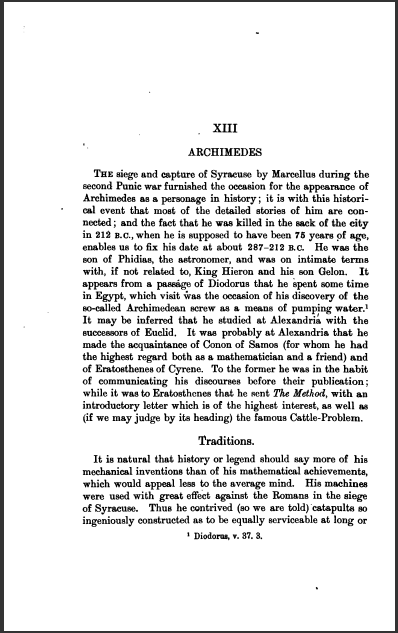
\includegraphics[width=0.6\textwidth]{./chapters/chapter04.png}
\end{figure}

\testsections


